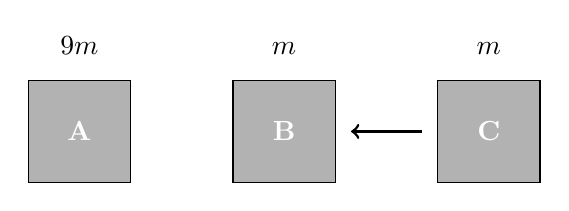
\begin{tikzpicture}[x=1cm,y=1cm]
  % block A, mass 9m
  \draw[fill=gray!60] (0,0) rectangle (1.3,1.3);
  \node[above] at (0.65,1.5) {$9m$};
  \node[white] at (0.65,0.65) {\textbf{A}};
  % block B, mass m
  \draw[fill=gray!60] (2.6,0) rectangle (3.9,1.3);
  \node[above] at (3.25,1.5) {$m$};
  \node[white] at (3.25,0.65) {\textbf{B}};
  % block C, mass m
  \draw[fill=gray!60] (5.2,0) rectangle (6.5,1.3);
  \node[above] at (5.85,1.5) {$m$};
  \node[white] at (5.85,0.65) {\textbf{C}};
  % arrow from C toward B
  \draw[->,line width=1pt] (5.0,0.65) -- (4.1,0.65);
\end{tikzpicture}
